\chapter{Tools}
\section{Git}
we will use \href{https://github.com/S61-Epsilon}{Github} for versioncontrol, this because it is easy to use and we are all familiar with it.

\section{Backlog}
for sprint planning we also use Github. so we have everything in one location \\

\begin{itemize} 
\item Scrumboard for \href{https://github.com/orgs/S61-Epsilon/projects/1}{Simulation}
\item Scrumboard for \href{https://github.com/orgs/S61-Epsilon/projects/2}{Java EE Application}
\end{itemize}
\newpage

\section{Sprint one planning}

\begin{figure}[h]
	\centering
	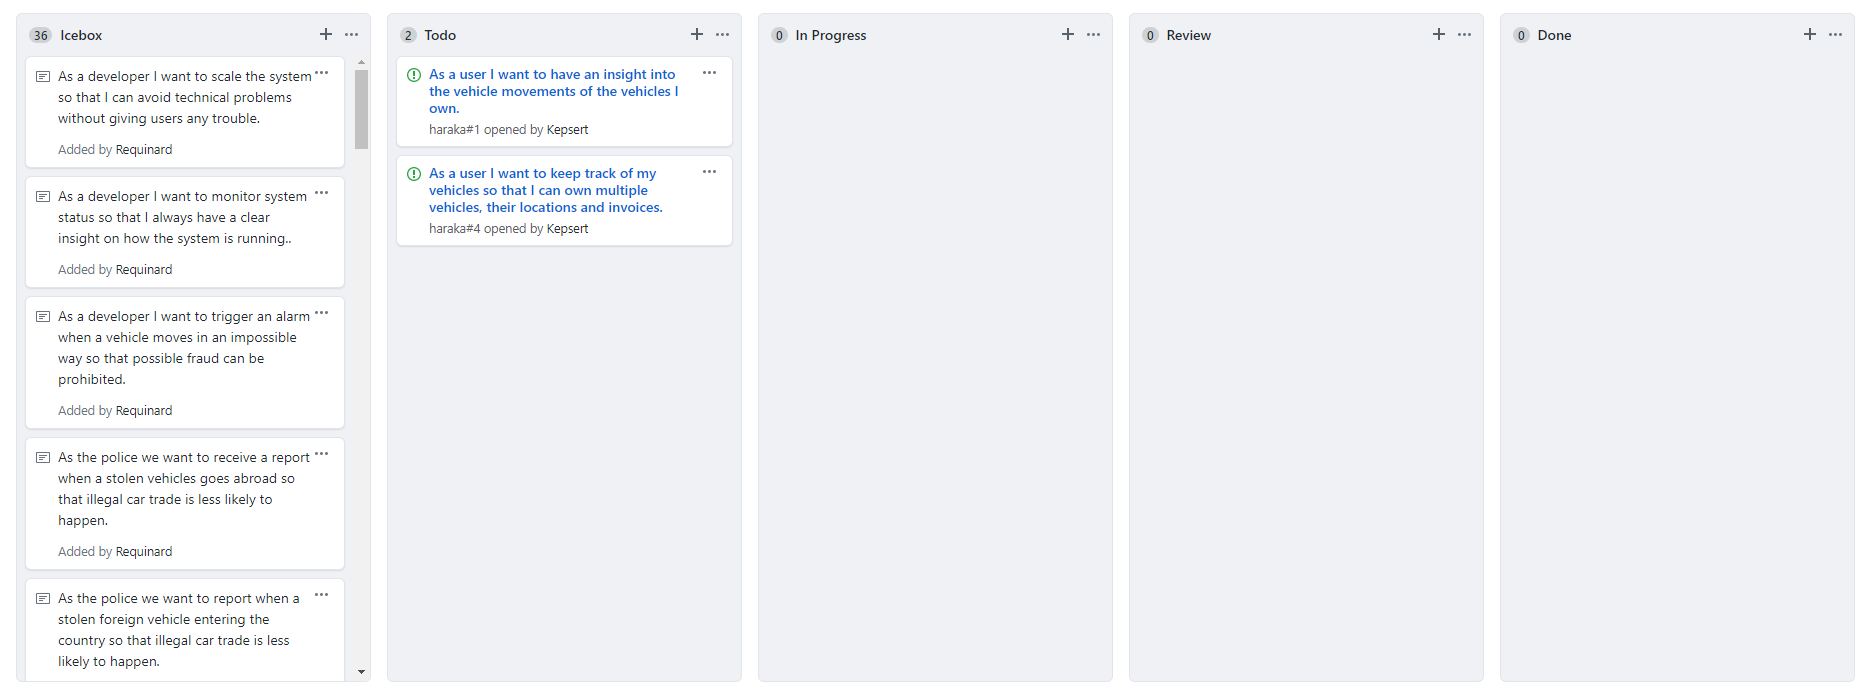
\includegraphics[width=1\linewidth]{Backlog_JavaEEApp}
	\caption{Backlog sprint one regarding the Java EE Application}
	\label{fig:backlogjavaeeapp}
\end{figure}

\begin{figure}[h]
	\centering
	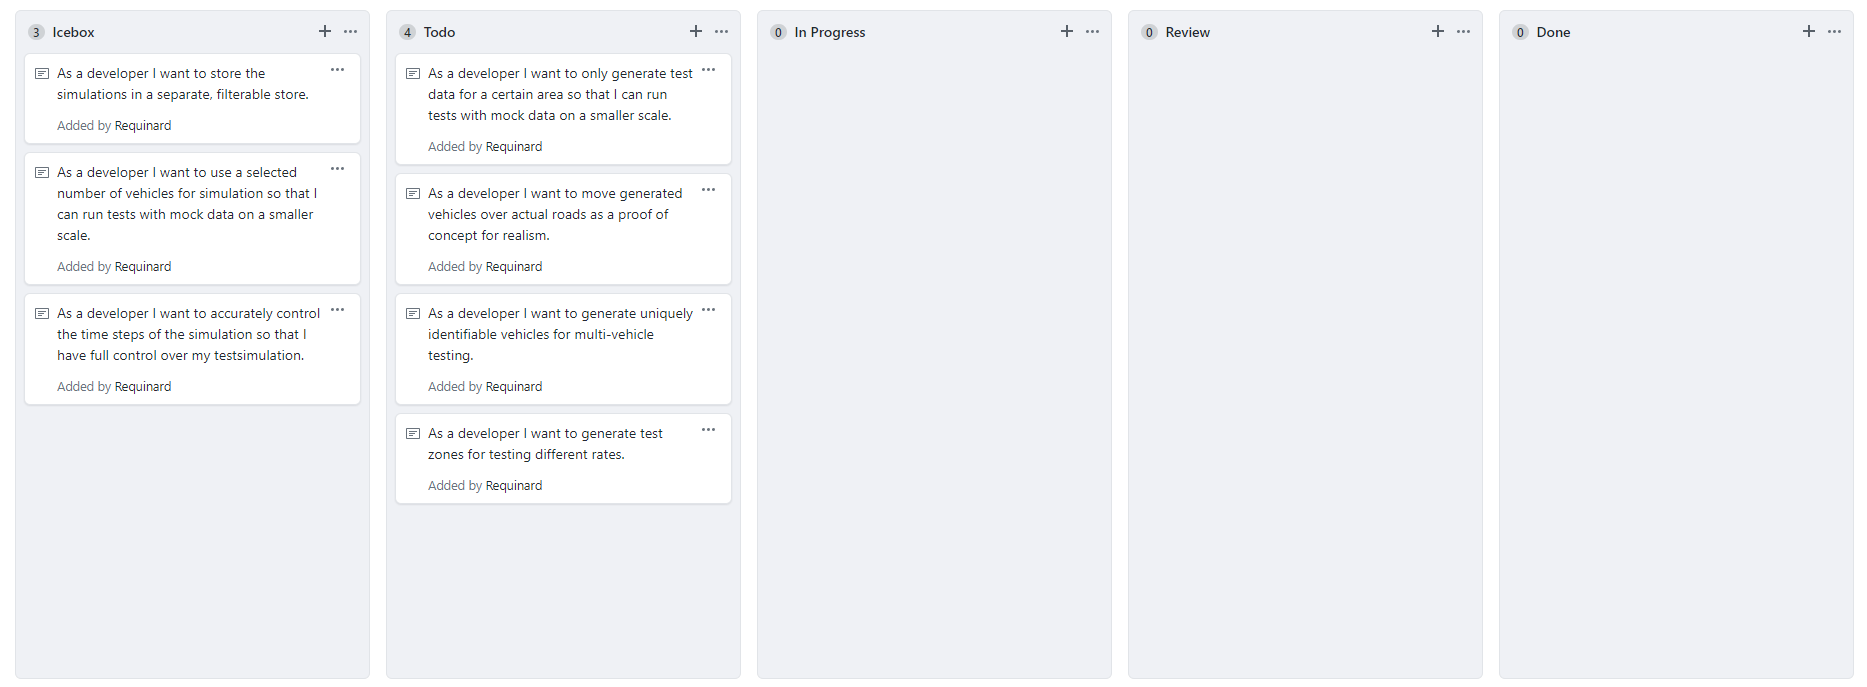
\includegraphics[width=1\linewidth]{Backlog_Simulation}
	\caption{Backlog sprint one regarding the Simulation}
	\label{fig:backlogsimulation}
\end{figure}

